\documentclass[%
12pt,
bachelor,    % тип документа
%natbib,      % использовать пакет natbib для "сжатия" цитирований
%subf,        % использовать пакет subcaption для вложенной нумерации рисунков
href,        % использовать пакет hyperref для создания гиперссылок
%colorlinks,  % цветные гиперссылки
%fixint,     % включить прямые знаки интегралов
%substylefile = bachelor.rtx
]{disser}%twoside, 

\usepackage[a4paper, includefoot, left=3cm, right=1cm, top=2cm, bottom=2cm, headsep=1cm, footskip=1cm]{geometry}

\usepackage[intlimits]{amsmath}
\usepackage{amssymb, amsfonts}

\usepackage[T2A]{fontenc}
\usepackage[utf8]{inputenc}
\usepackage[english,russian]{babel}
\ifpdf\usepackage{epstopdf}\fi
\usepackage[autostyle]{csquotes}

% Шрифт Times в тексте как основной
%\usepackage{tempora}
% альтернативный пакет из дистрибутива TeX Live
%\usepackage{cyrtimes}

% Шрифт Times в формулах как основной
%\usepackage[varg,cmbraces,cmintegrals]{newtxmath}
% альтернативный пакет
%\usepackage[subscriptcorrection,nofontinfo]{mtpro2}

\usepackage[%
style=gost-numeric,
backend=biber,
language=auto,
hyperref=auto,
autolang=other,
sorting=none
]{biblatex}
\addbibresource{biblio.bib}

% Плавающие рисунки "в оборку".
\usepackage{wrapfig}

% Номера страниц снизу и по центру
%\pagestyle{footcenter}
\chapterpagestyle{footcenter}

% Точка с запятой в качестве разделителя между номерами цитирований
%\setcitestyle{semicolon}

% Использовать полужирное начертание для векторов
\let\vec=\mathbf

% Включать подсекции в оглавление
\setcounter{tocdepth}{2}

\graphicspath{{fig/}}

\usepackage{comment}
\usepackage{textcomp}
\usepackage{tikz}
\usetikzlibrary{shapes,arrows}

\usepackage{setspace}
\onehalfspacing

% вставлять используемые пакеты сюда
% hyperref должен быть самым последним, иначе будут  баги с \chapter \section и \subsection

%\usepackage[
%pdfstartview   = FitH,
%bookmarksopen  = true,bookmarksopenlevel=0,
%plainpages     = false,pdfpagelabels,
%pagebackref    = false,
%pdftoolbar     = false,
%unicode,
%pdftex,
%hidelinks
%]{hyperref}

% Русские больше и меньше либо равно
\renewcommand{\leq}{\leqslant}
\renewcommand{\geq}{\geqslant}

\newtheorem{definition}{Определение}

% Больше переносов, меньше overflow hbox
%\tolerance=1000
%\hyphenpenalty=1000

\begin{document}
    \institution{%
        МИНОБРНАУКИ РОССИИ \\
        Федеральное государственное автономное образовательное учреждение высшего образования\\
        <<Национальный исследовательский университет\\
        <<Московский институт электронной техники>>\\
        Факультет Микроприборов и технической кибернетики\\% (МПиТК)
        Кафедра высшей математики №1% (ВМ-1)
    }
\title{Бакалаврская работа}
\topic{Оценка линейного искажающего оператора в задаче \\ восстановления изображения}%\normalfont\scshape 

\coursenum{01.03.04}
\course{Прикладная математика}
%\masterprog{Математические методы и моделирование\\ \>\ \ в естественнонаучной и технической сферах}
\author{~Терентьев И.~В.}
\group{ВМ-40}
\authorFullName{Терентьев Иван Владимирович}
%\apname{Прокофьев А.А.}

%Научник
\sa {Умняшкин С.~В.}
\sastatus{профессор, д.ф.-м.н.}
\city{Москва}
\date{2018}

\maketitle

%{\fontsize{13pt}{17}}
\tableofcontents
% MAIN BODY
\intro
В 2017 году у каждого второго в России есть смартфон\cite{mobileUsers}. 
Это значит, что у каждого второго россиянина есть маленькая камера, со значительными вычислительными ресурсами. Из-за несовершенства технической части, а именно малой светосилы, для уменьшения влияния шумов приходится увеличивать выдержку. В следствие чего при движении объекта или камеры на изображении возникает смаз. Это может стать причиной снижения информативности кадра. Кроме того широкое распространение получили экшн-камеры, которые специально созданы для работы в движении и тоже должны бороться со смазом.

Устранять проблему можно аппаратно: увеличивая площадь матрицы и светосилу объектива или программно~--- применяя алгоритмы восстановления изображений. Первый подход не применим для мобильных устройств, так как увеличивает размеры, вес и стоимость аппарата. Второй применить с каждым годом становится проще, так как растут вычислительные мощности устройств. Поэтому задача компенсации смаза является актуальной.
Пользователи смартфонов редко используют штативы для съёмки, поэтому аппарат испытывает тряску, как следствие изображение будет смазано. При этом в общем случае движение нелинейно и может быть представлено кривой линией.

В данной работе будут использованы итерационный метод Люси-Ричардсона для восстановления изображений и метод оценки параметров линейного искажающего оператора на основе кепстра изображения. Будут предложены дополнения и модификации алгоритма для более точной реконструкции искажённого кадра. Также будет предложен алгоритм оценки криволинейного искажающего оператора с модификациями.

Целью представленной работы является разработка метода оценки параметров  криволинейного смаза изображения, с последующим восстановлением изображения методом Люси-Ричардсона. Для достижения этой цели предстоит решить следующие задачи:

\begin{itemize}
\item разработать метод оценки параметров искажения;
\item определить критерий качества восстановленного изображения и искажающего оператора
\item реализовать алгоритм, который будет принимать на вход искажённое изображение и возвращать оценку неискажённого изображения.
\end{itemize}

В первой главе рассмотрены теория, описывающая модель искажения, методы оценки его параметров и устранения.

Во второй главе описываются программные решения, с помощью которых происходит оценка качества работы алгоритмов, определение параметров смаза.

В третьей главе приводятся результаты экспериментов и выводы по результатам работы.
\chapter{Обзор проблематики восстановления изображений}
\section{Модель искажения}\label{seqtion:distortionModel}
Изображение~--- это двумерная проекция трёхмерной сцены. Записывающая система(камера) проецирует сцену на двумерную область~--- изображение. Под изображением понимаем двумерный дискретный сигнал $f(x,y)$, где $0\leq x \leq M$, $0\leq y\leq N$ ($M$, $N$~--- ширина и высота изображения соответственно). В данной работе рассматриваем только обработку полутоновых изображений со значениями яркости $0\leq f(x,y)\leq 1$.

\begin{figure}[h!]
	\tikzset{%
		block/.style    = {draw, thick, rectangle, minimum height = 3em,
			minimum width = 3em, node distance = 3cm},
		sum/.style      = {draw, circle, node distance = 3cm}, % Adder
		input/.style    = {coordinate}, % Input
		output/.style   = {coordinate, node distance = 3cm} % Output
	}
    \centering
    \begin{tikzpicture}[auto, thick, node distance=2cm, >=triangle 45]
    \draw
        node [input, name=in] {} 
        node [block, right of=in] (hxy) {$h(x,y)$}
        node [sum, right of=hxy] (sum1) {\Large$+$}
        node [input, above of=sum1] (noize) {}
        node [output, right of=sum1] (out){$g(x,y)$};
    \draw[->](in)     -- node {$f(x,y)$}(hxy);
    \draw[->](hxy)    -- node {$s(x,y)$}(sum1);
    \draw[->](noize)  -- node {$\eta(x,y)$}(sum1);
    \draw[->](sum1)   -- node {$g(x,y)$}(out);
    \end{tikzpicture}
    \caption{Линейная система искажения изображения}
    \label{fig:distortionScheme}
\end{figure}

Пусть $f(x,y)$~--- исходное <<правильное>> изображение; $g(x,y)$~--- изображение подвергнутое искажению; $h(x,y)$~--- импульсная характеристика (ИХ) оператора искажения; $\hat{f}(x,y)$~--- оценка неискажённого изображения $f(x,y)$; $\eta(x,y)$~--- некоррелированный гауссов шум. Обозначим $F(u,v)$, $G(u,v)$, $H(u,v)$, $N(u,v)$ Фурье-образы функций $f(x,y)$, $g(x,y)$, $h(x,y)$ и $\eta(x,y)$ соответственно, полученные дискретным преобразованием Фурье~\cite[стр.~332]{gonsalesDigital2012}.
Допускаем, что процесс формирования искажённого изображения $g(x, y)$ линейный и его можно описать с помощью линейной дискретной системы~\cite[стр.~403]{gonsalesDigital2012}
\begin{equation}\label{eq:distortion}
g(x, y) = h(x,y) \conv f(x,y) + \eta(x,y),
\end{equation}
где $<\conv>$~--- операция двумерной свёртки изображения $f(x,y)$ размером $M\times N$ с импульсной характеристикой фильтра $h(x,y)$ размером $m\times n$, которая описывается следующим выражением~\cite[стр.~298]{gonsalesDigital2012}:

\begin{equation}
h(x,y) \conv f(x,y) = \sum_{s=-a}^{a}\sum_{t=-b}^{b}h(s,t)f(x-s, y-t),
\end{equation}
где $a=(m-1)/2$ и $b = (n-1)/2$.

\begin{definition}\label{def:impulseResponse}
Двумерная \textbf{импульсная характеристика} (или функция рассеяния точки, \textbf{ФРТ}) — это реакция двумерной дискретной системы на единичный импульс $\delta$:
$$\delta(n,m) = 
	\begin{cases}
		1, &n=m=0\\
		0, &n\ne 0, m\ne 0
	\end{cases}$$
\end{definition}

Таким образом, процесс искажения изображения описывается как результат взаимодействия исходного изображения $f(x, y)$ с линейно-дискретной системой, изображённой на рисунке~\ref{fig:distortionScheme}. Сигнал $f(x, y)$ подвергается воздействию оператора смаза с импульсной характеристикой $h(x, y)$ , которая обычно не известна заранее. Из-за внешних факторов и несовершенства съёмки к искажению добавляется шум, который считается некоррелированным случайным процессом, также некоррелированным с изображением.

В частотной области процесс искажения~(\ref{eq:distortion}) выглядит следующим образом:
\begin{equation}\label{eq:distortionFourier}
G(u,v) = H(u,v)\cdot F(u,v) + N(u,v),
\end{equation}
так как операция свёртки в пространственной области эквивалентна умножению в частотной области~\cite[стр.~39]{basicsOfDigitalDataProcessing2016Umnyashkin}

Смаз на изображении всегда возникает при относительном движении камеры и объекта. Для определения импульсной характеристики оператора искажения, рассмотрим случай, когда камера перемещается с постоянной горизонтальной скоростью относительно сцены. В дискретном случае~\cite{iterableImageRestorationBiemonLangdeik}:
\begin{equation}\label{eq:horizontalBlurPsf}
	h(x,y) = 
		\begin{cases}
			\frac{1}{L+1}, & 0 \leq y \leq L, x=0\\
			0,             & \text{в остальных случаях},
		\end{cases}
\end{equation}
где \textit{L}~--- величина смаза, то есть количество точек(пикселей), на которое сместилось изображение соответствующих одной точке объекта. Выражение (\ref{eq:horizontalBlurPsf})~--- один из вариантов функции рассеяния точки.

Частотная характеристика данного оператора искажения определяется выражением~\cite{iterableImageRestorationBiemonLangdeik}:

\begin{equation}\label{eq:horizontalBlurIRFourier}
H(u,v) =       
	\frac{1}{L+1}e^{-i\frac{L\pi}{N}u}\frac{\sin\frac{\pi(L+1)u}{N}}{\sin\frac{\pi u}{N}}
\end{equation}

На рисунке (\ref{fig:linearPsf}) изображены импульсная и частотная характеристики смаза в 30 пикселей под углом $300^\circ$. Частотная характеристика состоит из параллельных линий с углом наклона $30^\circ$. Амплитудно-частотная характеристика (\ref{eq:horizontalBlurIRFourier}) имеет нули в точках $\frac{N}{L+1}k, v$, где $k = \pm 1, \pm2, ...$. Таким образом, на рисунке~\ref{fig:linearPsfFourier} расстояние между параллельными линиями равно $N/30$. Угол наклона линий на рисунке~\ref{fig:linearPsfFourier} характеризует угол смаза~\cite{iterableImageRestorationBiemonLangdeik}.
\begin{figure}[h!]
	\centering
	\begin{subfigure}[b]{0.45\textwidth}
		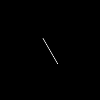
\includegraphics[width=\textwidth]{linear-psf-arr}
		\caption{импульсная характеристика}
		\label{fig:linearPsfArr}
	\end{subfigure}%
	\hfill
	\begin{subfigure}[b]{0.45\textwidth}
		
\includegraphics[width=\textwidth]{linear-psf-fourier}%width=\linewidth
		\caption{амплитудно-частотная характеристика}
		\label{fig:linearPsfFourier}
	\end{subfigure}%
	\caption{Смаз величиной в 30 пикселей под углом $300^{\circ}$}\label{fig:linearPsf}
\end{figure}

\section{Методы восстановления изображения}
Так как в процессе искажения основная операция~--- свёртка, то процессы восстановления изображения основанные на обращении данной операции называются \textit{деконволюцией}. Методы деконволюции разделяются на два класса: итерационные и неитерационные.

Для сравнения исходного и восстановленного изображений $I_1, I_2$ будем использовать две метрики, среднеквадратичную ошибку(СКО) или MSE(mean square error) и пиковое отношение сигнала к шуму PSNR(peak signal to noise ratio) в дБ, которое определим через MSE: 
\begin{equation}\label{eq:mse}
MSE = \frac{1}{MN}\sum_{i=0}^{M-1}\sum_{j=0}^{N-1}\left| I_1(i,j)-I_2(i,j)\right|^2
\end{equation}
\begin{equation}\label{eq:psnr}
PSNR = 20\log_{10}\left(\frac{MAX_I}{\sqrt{MSE}}\right), \text{дБ},
\end{equation}
где $MAX_I$~--- максимальная яркость исходного изображения.

Перед восстановлением, для избежания дребезга края искажённых изображений размываются функцией \verb|edgetaper|.

\subsection{Инверсная фильтрация}
\textit{Инверсная фильтрация}~--- простейший метод восстановления, исходя из модели искажения представленной в частотной области (\ref{eq:distortionFourier}) предполагает следующую оценку спектра восстановленного изображения $\hat{F}(u,v)$~\cite[стр.~411]{gonsalesDigital2012}:
\begin{equation}\label{eq:inverseFiltrationFourier}
\hat{F}(u,v) = \frac{G(u,v)}{H(u,v)}.
\end{equation}
Из (\ref{eq:distortionFourier}) и (\ref{eq:inverseFiltrationFourier}) следует, что
\begin{equation}\label{eq:inverseFiltration}
\hat{F}(u,v) = F(u,v) + \frac{N(u,v)}{H(u,v)}
\end{equation}

Инверсная фильтрация не пригодна для восстановления зашумленных изображений: на частотах, где спектр искажающего оператора близок к нулю второе слагаемое (\ref{eq:inverseFiltration}) вносит очень большой вклад в сумму и как следствие искажает ещё больше оценку исходного изображение.
\begin{figure}[h!]
	\begin{subfigure}[b]{0.5\textwidth}
		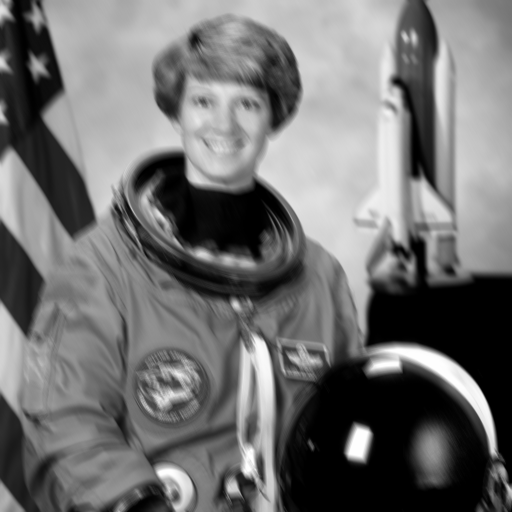
\includegraphics[width=\linewidth]{deconv-astro-shift15}
		\caption{искажённое изображение~--- сдвиг \\на 15 пикселей, шум $\sigma=10^{-5}$}
		\label{fig:astroShift15}
	\end{subfigure}%
	\begin{subfigure}[b]{0.5\textwidth}
		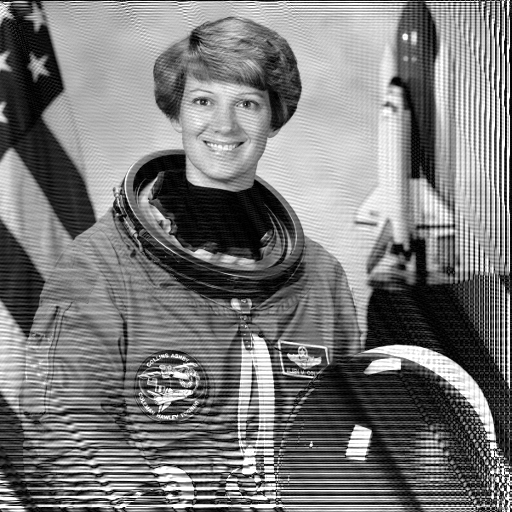
\includegraphics[width=\linewidth]{deconv-inverse-filter}
		\caption{восстановленное изображение\\ PSNR=17.93дБ}
		\label{fig:astroInverseRestored}
	\end{subfigure}%
	\caption{Восстановление изображения размером $512\times 512$ c помощью инверсной фильтрации. Параметры искажения: смаз~--- 15 пикселей, угол $300^\circ$, шум~--- $\sigma_\eta=10^{-5}$}
\end{figure}

При этом шума в камере избежать невозможно: как бы ни была дорога аппаратура, от теплового шума не избавиться.

\subsection{Фильтр Винера}
Основной недостаток инверсной фильтрации~--- неспособность корректно восстанавливать зашумлённые изображения. Чтобы бороться с ним был разработан, в частности, метод \textit{винеровской фильтрации}, использующий свойства функции рассеяния. Основная идея этого алгоритма деконволюции заключается в следующем: изображение и шум рассматриваются как случайные процессы. Ставится следующая задача: необходимо найти такую оценку $\hat{f}$ для исходного изображения $f$, чтобы среднеквадратичное отклонение $e$ этих величин друг от друга было минимальным.

Выполнение этих условий на практике сходится к следующей формуле:
\begin{equation}\label{eq:wiener}
\hat{F}(u,v)=\left(\frac{1}{H(u,v)}\frac{|H(u,v)|^2}{|H(u,v)|^2+K}\right)G(u,v),
\end{equation}
где $K$~--- эмпирически определяемая константа, выбирается так, чтобы получить наилучшее качество восстановления.

\begin{figure}[h!]
	\begin{subfigure}[b]{0.5\textwidth}
		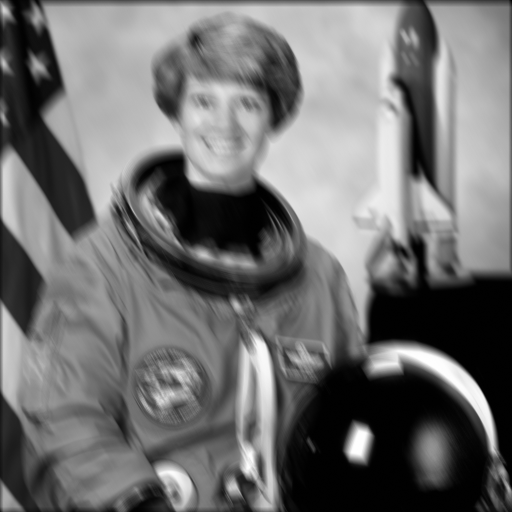
\includegraphics[width=\linewidth]{deconv-shift15}
		\caption{искажённое изображение~--- сдвиг \\на 15 пикселей}
		\label{fig:astroShift15u}
	\end{subfigure}%
	\begin{subfigure}[b]{0.5\textwidth}
		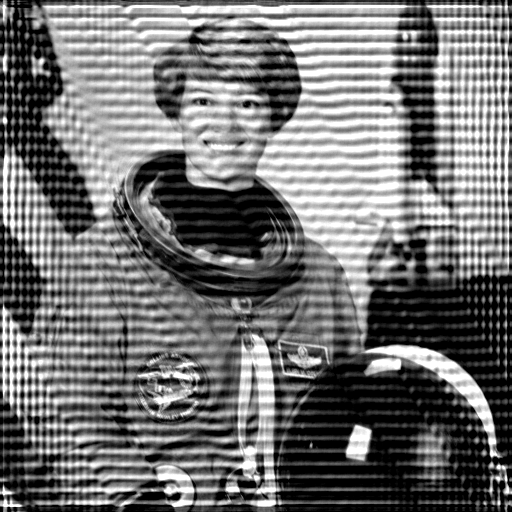
\includegraphics[width=\linewidth]{deconv-shift15-restored-u-wiener}
		\caption{восстановленное изображение\\ PSNR=23.02дБ}
		\label{fig:astroWienerRestored}
	\end{subfigure}%
	\caption{Восстановление изображения размером $512\times 512$ c помощью винеровской фильтрации. Параметры искажения: смаз~--- 15 пикселей, угол $300^\circ$, шум~--- $\sigma_\eta=10^{-3}$}
\end{figure}

На практике не всегда получается получить удовлетворительный результат с помощью выражения (\ref{eq:wiener}). Это происходит из-за того что значения спектров шума и сигнала не известны, а оценка K может быть ошибочна. Кроме того не всегда возможно подбирать этот параметр вручную.

\subsection{Регуляризация по Тихонову}
Существуют методы, для использования которых достаточно знать только среднее значение шума и его дисперсию. Один из таких методов~--- \textit{регуляризация по Тихонову}. Этот метод в спектральной области описывается соотношением~\cite[стр.~418]{gonsalesDigital2012}:
\begin{equation}\label{eq:tikhonov}
\hat{F}(u,v) = \left(\frac{H^*(u,v)}{|H(u,v)|^2 + \gamma|P(u,v)|^2}\right)G(u,v)
\end{equation}

В этом методе от выбора параметра регуляризации $\gamma$ (его выбирают эмпирически или итеративно) зависит качество восстановленного изображения. $P(u,v)$~--- двумерное ДПФ дискретного аналога оператора Лапласа $\nabla^2 = \left(\frac{\partial^2}{\partial x^2} + \frac{\partial^2}{\partial y^2}\right)$:
\begin{equation}
p(x,y) = \begin{bmatrix}
		0 & 1 & 0\\
		1 &-4 & 1\\
		0 & 1 & 0
	\end{bmatrix}
\end{equation}

При $\gamma = 0$ метод вырождается в инверсную фильтрацию. Пример работы алгоритма представлен на рисунке~\ref{fig:tikhonov}
\begin{figure}[h!]
	\begin{subfigure}[b]{0.5\textwidth}
		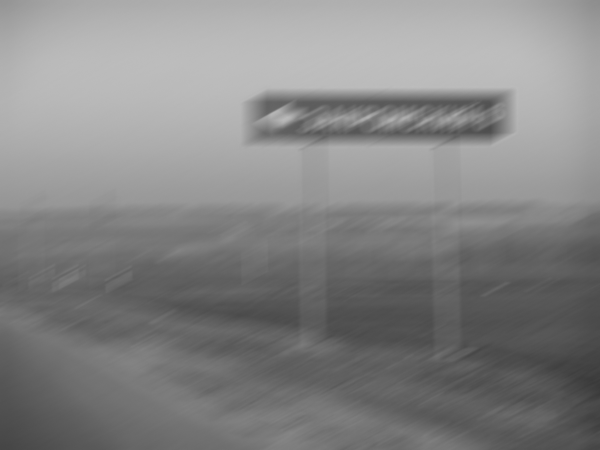
\includegraphics[width=\linewidth]{zakromsky-shift20}
		\caption{искажённое изображение~--- сдвиг \\на 20 пикселей}
		\label{fig:zakromskiyShift20}
	\end{subfigure}%
	\begin{subfigure}[b]{0.5\textwidth}
		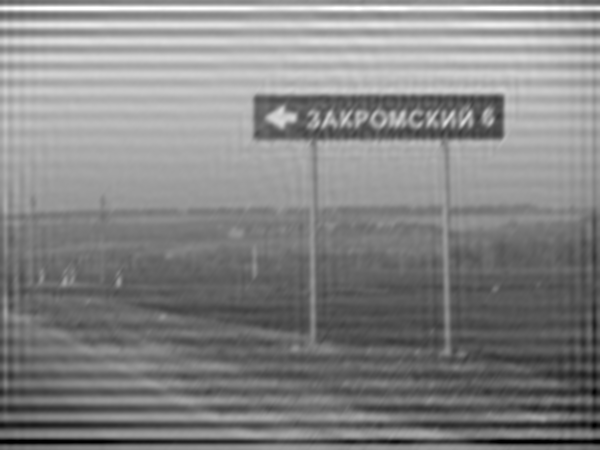
\includegraphics[width=\linewidth]{zakromsky-shift20-tikhonov}
		\caption{восстановленное изображение\\ PSNR=45дБ}
		\label{fig:zakromskiyShift20Tikhonov}
	\end{subfigure}%
	\caption{Восстановление изображения размером $450\times 600$ c помощью регуляризации по Тихонову. Параметры искажения: смаз~--- 20 пикселей, угол $56^\circ$, шум~--- $\sigma_\eta=0.003$}
	\label{fig:tikhonov}
\end{figure}

\subsection{Метод Люси-Ричардсона}
Выше были приведены неитерационные методы. Их недостатком является то, что результат работы сильно зависит от точности определения ИХ $h(x,y)$. Поэтому всё чаще применяются итерационные методы восстановления, которые в процессе работы уточняют ИХ, хотя и требуют больших вычислительных ресурсов. Один из таких методов был предложен независимо друг от друга Л.~Б.~Люси(1974)~\cite{lucy} и В.~Х.~Ричардсоном (1972)~\cite{richardson}. Этот подход основан на использовании метода максимального правдоподобия для изображения, моделируемого в виде статистик Пуассона. Формула для оценки неискажённого изображения $\hat{f}_{k+1}(x,y)$ на $(k + 1)$-ой итерации в \textit{методе Люси-Ричардсона} выглядит следующим образом:
\begin{equation}\label{eq:lucy}
	\hat{f}_{k+1}(x,y) = \hat{f}_k(x,y) \left(h(-x,-y) \conv \frac{g(x,y)}{h(x,y) \conv \hat{f}_k(x,y)}\right)
\end{equation}

Позже были предложены модификации метода Люси-Ричардсона~\cite{richardsonLucyModifiedBiggs}, направленные на увеличение его скорости сходимости и качества восстановленного изображения. В данной работе применяется метод Люси-Ричардсона с модификациями (\ref{eq:lucyMod1} и \ref{eq:lucyMod2}).
\begin{equation}\label{eq:lucyMod1}
	\hat{f}_k=u_k+\alpha_k h_k,
\end{equation}
где $h_k = u_k - u_{k-1}$, $u_k = \hat{f}_k + g_k$, $g_k = \phi(\hat{f}_k)-\hat{f}_k$, $\phi(\hat{f}_k)$~--- результат $(k+1)$-ой итерации алгоритма Люси-Ричардсона~(\ref{eq:lucy}). Эта модификация призвана ускорить работу метода, используя экстраполяцию оценки изображения.   
\begin{equation}\label{eq:lucyMod2}
	\hat{f}_k=\hat{f}_k \cdot C,
\end{equation}
где $C$ — модифицированное ядро Люси-Ричардсона. Ядро $C$ находится следующим образом:
\begin{equation}
	C = p(x,y)^{\gamma-1}\cdot (\gamma-(\gamma-1)p(x,y)),
\end{equation}
где
\begin{equation}
	p(x,y) = \min\left[
		-\frac{2}{t^2}\left(
			g(x,y)\ln\frac{g(x,y)}{J(x,y)}-J(x,y)+g(x,y)
		\right), 1
	\right],
\end{equation}
а $t$~--- пороговое значение, которое определяет уровень затухания(обычно выбирают $t=\sigma/10$, где $\sigma$~--- СКО шума участвующего в искажении исходного изображения), $J(x,y) =h(x,y) \conv \hat{f}_k(x,y)$~--- оценка искажённого изображения. Из эмпирических соображений обычно выбирают $\gamma=10$. Данная модификация повышает точность и сходимость метода. 

\begin{figure}[h!]
	\begin{subfigure}[b]{0.45\textwidth}
		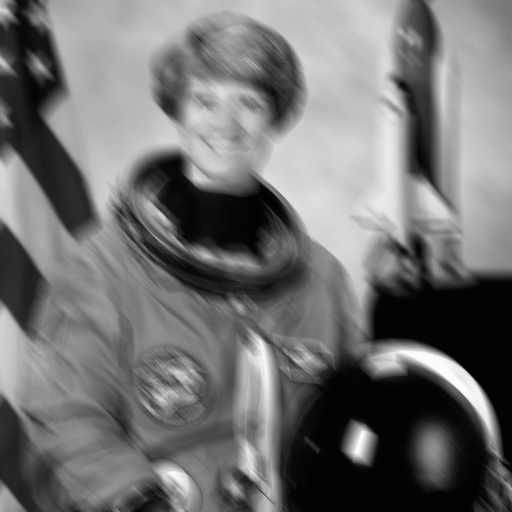
\includegraphics[width=\linewidth]{richardson-lucy-astro-distorted}
		\caption{искажённое изображение~--- сдвиг \\на 20 пикселей}
		\label{fig:astroLucyBlurred}
	\end{subfigure}%
	\hfill
	\begin{subfigure}[b]{0.45\textwidth}
		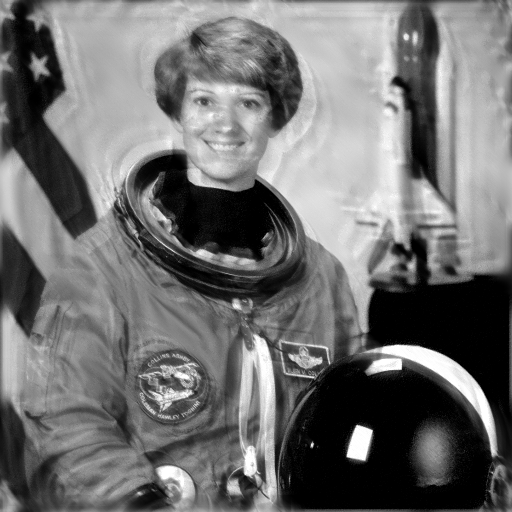
\includegraphics[width=\linewidth]{richardson-lucy-astro-distorted-restored}
		\caption{восстановленное изображение\\ PSNR=21.77дБ}
		\label{fig:astroLucyRestored}
	\end{subfigure}%
	\caption{Восстановление изображения размером $512\times 512$ c помощью метода Люси-Ричардсона. Параметры искажения: смаз~--- 20 пикселей, угол $45^\circ$, шум~--- $\sigma_\eta=0.003$}
	\label{fig:richardsonLucy}
\end{figure}

На рисунке~\ref{fig:richardsonLucy} показан пример работы модифицированного метода Люси-Ричардсона. Как видим, результат работы итерационного метода по качеству превосходит результаты неитерационных методов.


\begin{comment}
%%% не работает без известнй ИХ 
\subsection{Слепая деконволюция}
\end{comment}

\section{Постановка задачи оценки искажающего оператора}
Были рассмотрены несколько методов восстановления изображения. Все они для работы требуют предварительно получить значение ИХ искажающего оператора. Однако в реальных задачах оператор обычно неизвестен и не всегда может быть оценён из параметров сцены. Следовательно необходимо  <<уметь>> получать оценку ИХ из искажённого изображения. Так как метод Люси-Ричардсона на использованных изображениях показал себя лучше других методов, в дальнейшем для процесса деконволюции будем рассматривать только его, а усилия сконцентрируем на создании метода оценки искажающего оператора.
\begin{definition}\label{def:bestPsfEstimaton}
	Наилучшей оценкой $h^*$ искажающего оператора $h$ назовём такую, при использовании которой MSE восстановленного изображения $\hat{f}$ будет минимальна.
	\begin{equation}\label{eq:bestPsf}
	\hat{h}^* = \argmin_{\hat{h}}MSE(f, \hat{f}(g,\hat{h})),
	\end{equation}
\end{definition}
где $\hat{f}(g,h)$~--- оценка восстановленного изображения полученная применением модифицированного метода Люси-Ричардсона к искажённому изображению с оценкой искажающего оператора~$\hat{h}$. 

\chapter{Метод оценки линейного искажающего оператора}
\section{Нахождение параметров искажения}
Как было сказано ранее, для восстановления изображения необходимо определить искажающий оператор. Он представляется дискретной импульсной характеристикой(ИХ). Однако такое представление не самое удачное для поиска, потому что имеет слишком большое количестве степеней свободы. Для эффективного поиска необходимо построить более удобную модель, задающую оператор ограниченным количеством параметров.

ИХ для вычислений представляется в виде матрицы. Простейшее представление смаза~--- линейный смаз~(\ref{eq:horizontalBlurPsf}).
\begin{equation}\label{eq:linearBlurArray}
\begin{pmatrix}
0 & 0 & 0 & 0.092 & 0.024\\
0 & 0.22 & 0.181 & 0.213 & 0.024\\
0.121 & 0.255 & 0.038 & 0 & 0\\
0.061 & 0 & 0 & 0 & 0
\end{pmatrix}
\end{equation}

Так например представляется в ИХ смаза длиной в 5 пикселей под углом $30^\circ$
\subsection{Кепстральный метод оценки линейного оператора}
Линейный смаз представляется величиной и углом смаза, альтернативное представление: координаты вектора смаза. Как уже было сказано ранее в разделе~(\ref{seqtion:distortionModel}), по спектру искажённого изображения визуально можно приблизительно оценить величину и угол смаза.
\begin{figure}[h!]
	\centering
	\begin{subfigure}[t]{0.3\textwidth}
		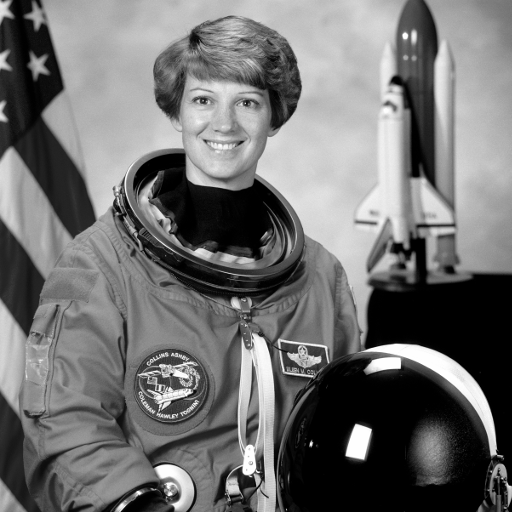
\includegraphics[width=\linewidth]{astro}
		\caption{исходное изображение}
	\end{subfigure}
	\hfill
	\begin{subfigure}[t]{0.3\textwidth}
		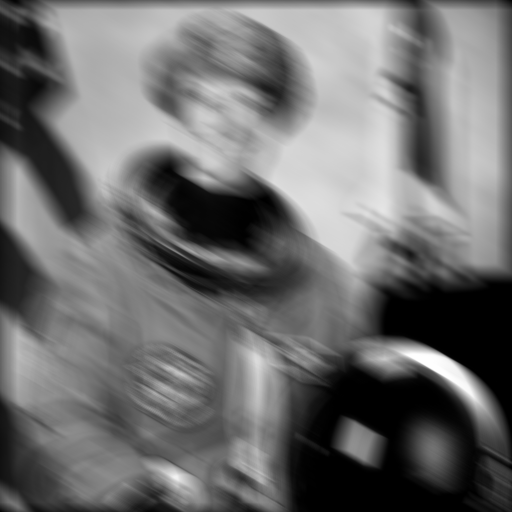
\includegraphics[width=\linewidth]{deconv-astro-blurred-shift40}
		\caption{смазанное изображение}
		\label{fig:astroShift40}
	\end{subfigure}%
	\hfill
	\begin{subfigure}[t]{0.3\textwidth}
		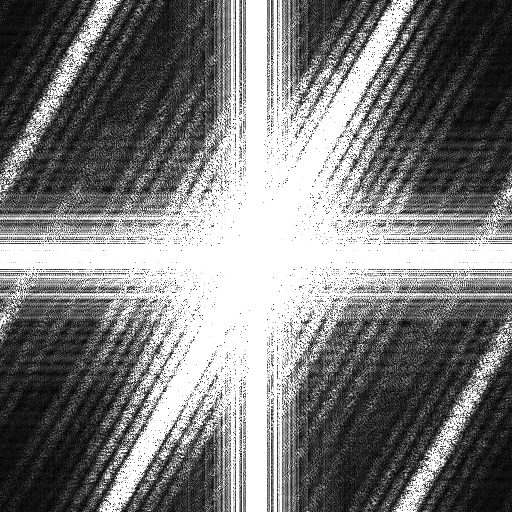
\includegraphics[width=\linewidth]{deconv-astro-spectre-shift40}
		\caption{спектр смазанного изображения}
		\label{fig:astroShift40Spectre}
	\end{subfigure}
	\caption{Смаз величиной в 40 пикселей под углом $330^{\circ}$}
	\label{fig:spectre}
\end{figure}

На рисунке~\ref{fig:spectre} представлены оригинальное изображение, исходное изображение подвергнутое смазу и спектр смазанного изображения. По спектру (рис.~\ref{fig:astroShift40Spectre}) расстояние между чёрными полосами, в которых значение спектра близко к нулю является обратным к величине смаза. Данные полосы ортогональны вектору смаза, угол наклона которого равен $330^\circ$. Однако, определение точных значений этих величин по частотному представлению изображения затруднительно. Для корректной работы методов восстановления изображения важно как можно точнее оценить ФРТ. Поэтому используют более точные способы определения параметров смаза.

Один из таких методов оценки параметров оператора линейного смаза основан на использовании кепстра изображения $\hat{f}(x,y)$~\cite{iterableImageRestorationBiemonLangdeik}
\begin{definition}\label{def:kepstr}
	\textbf{Кепстром} $\hat{f}(x,y)$ изображения называют обратное преобразование Фурье логарифма модуля преобразования Фурье изображения.
	\begin{equation}
	\hat{g}(x,y) = F^{-1}\{log|F(u,v)|\},
	\end{equation}
\end{definition}
где $F^{-1}\{\cdot\}$~--- обратное преобразование Фурье, а $F(u,v)$~--- частотное представление изображения. Название <<кепстр>> получено перестановкой первых четырёх букв слова <<спектр>>.

Одним из основных свойств кепстра является то, что при свёртке двух сигналов их кепстры складываются. Таким образом, если
\begin{equation}
	g(x,y) = h(x,y) \conv f(x,y),
\end{equation}
то \cite{iterableImageRestorationBiemonLangdeik}
\begin{equation}\label{eq:kepstrSum}
	\hat{g}(x,y) = \hat{h}(x,y) + \hat{f}(x,y)
\end{equation}

При горизонтальном размытии ЧХ искажения можно записать в виде~(\ref{eq:horizontalBlurIRFourier}):
\begin{equation*}
H(u,v) =       
\frac{1}{L+1}e^{-i\frac{L\pi}{N}u}\frac{\sin\frac{\pi(L+1)u}{N}}{\sin\frac{\pi u}{N}}
\end{equation*}
Она имеет нули в точках $\frac{N}{L+1}k, v$, где $k$~--- ненулевое целое, поэтому $\hat{h}(x,y)$ имеет большой отрицательный пик на расстоянии $L$ от начала координат. Следовательно у кепстра искажённого изображения он тоже будет, что сообщает о наличии искажения и его параметрах.
\begin{figure}[h!]
	\centerline{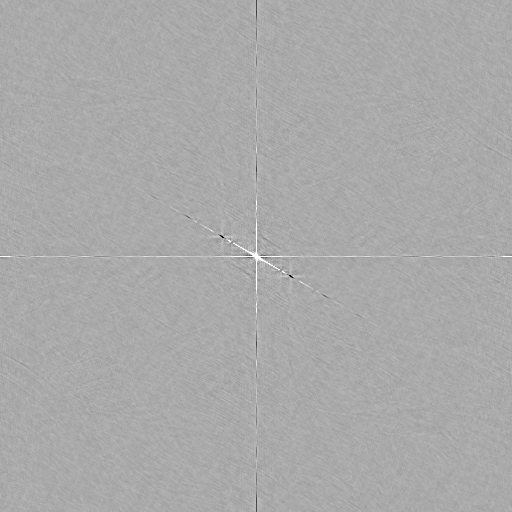
\includegraphics[width=0.5\linewidth]{deconv-kepstr-shift40-pi6}}
	\caption{Кепстр изображения смазанного на 40 пикселей под углом $330^{\circ}$.}
	\label{fig:kepstr}
\end{figure}

На рисунке~\ref{fig:kepstr} изображён кепстр искажённого изображения~\ref{fig:astroShift40}. В центре находится точка $(0,0)$. Симметрично относительно неё расположены тёмные точки, соответствующие отрицательным пикам, характеризующим параметры смаза. Их координаты соответствуют вектору смаза. Таким образом можно достаточно точно определить искажение. Отклонение от реальных значений достигает 1-2 пикселей.

\begin{figure}[h!]
	\centerline{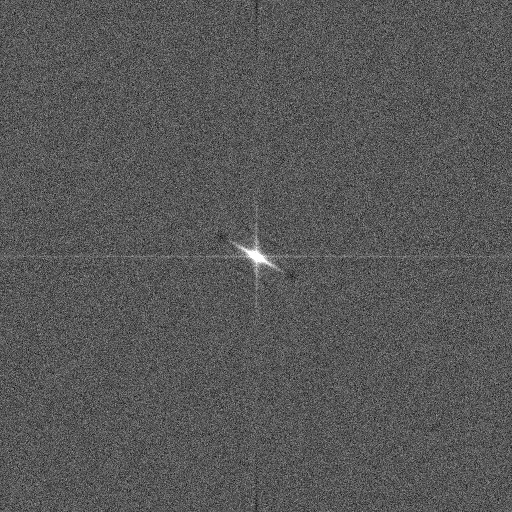
\includegraphics[width=0.5\linewidth]{deconv-kepstr-noised-shift40-pi6}}
	\caption{Кепстр изображения смазанного на 40 пикселей под углом $330^{\circ}$, зашумлённого с $\sigma=0,1$.}
	\label{fig:kepstrNoised}
\end{figure}
%%%% сослаться на диплом Кристины? Не это: ~\cite{panfilovaLinearBlur}
Кепстральный метод обладает рядом недостатков: в случае небольшого искажения (длина вектора размытия меньше 5 пикселей), точное определения смаза становится затруднительным. Также проблематично определить вектор смаза при большом шуме($\sigma_\eta \geq 5\cdot 10^{-2}$)~\cite{panfilovaThesis} Так как вклад шума слишком велик, минимум спектра приходится на случайную составляющую спектра, что видно на рисунке~\ref{fig:kepstrNoised}.

\subsection{Уточнение параметров искажения}
Кепстральный метод находит только целочисленные координаты вектора сдвига, при этом возможна погрешность в несколько пикселей, тогда как на практике величина смаза есть число вещественное. Ниже будет рассмотрен алгоритм, позволяющий уточнить параметры смаза.

Найти наилучшую оценку искажающего оператора~(\ref{eq:bestPsf}) невозможно, так как исходное изображение в общем случае неизвестно. Вместо этого можно минимизировать целевую функцию, а именно MSE конволюции оценки изображения и искажающего оператора относительно искажённого изображения. Тогда искомая ИХ $\hat{h}^*$ будет найдена по следующей формуле:
\begin{equation}\label{eq:bestPsfModified}
\hat{h}^* = \argmin_{\hat{h}} MSE(g, \phi(g,\hat{h}) \conv \hat{h}),
\end{equation}
где $\phi(g, h)$~--- результат применения деконволюции(используем метод Люси-Ричардсона) с оператором $h$.

Так как ИХ линейного смаза $h_{x_h,y_h}(x,y)$описывается координатами вектора смаза, минимизировать будем функцию двух переменных $x_h, y_h$.

%%%%%%%%%%%%%%%%%%%%%%%%%%%%%%%%%%%%%%%%%%%%%%%%%%%%%%%%
\section{Нахождение параметров криволинейного искажающего оператора}

\subsection{Представление криволинейного искажающего оператора}
Представление смаза отрезком~--- удобно, но не всегда отражает действительность. В общем случае смаз криволинеен.

\begin{figure}[h!]
	\centering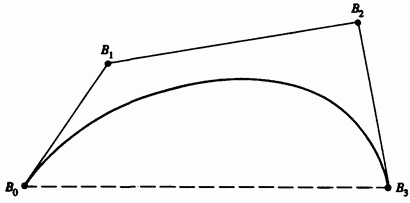
\includegraphics[width=0.5\linewidth]{bezier-curve-polygon-from-book}
	\caption{Кривая Безье и определяющие её точки.}
	\label{fig:bezierPolygon}
\end{figure}

Пьер Безье предложил метод создания кривых и поверхностей любой формы. Безье вывел математическую основу своего метода из геометрических соображений. Кривая Безье задаётся многоугольником как показано на рисунке~\ref{fig:bezierPolygon}.~\cite{mathBasicsOfCopmuterGraphics}.
Математическое представление кривой Безье имеет вид:
\begin{equation}
P(t) = \sum_{i=0}^{n} B_i J_{n,i}(t),\ 0\leq t \leq 1,
\label{eq:bezierCurveN}
\end{equation}
где $B_i, i=0\dots n-1$~--- точки многоугольника Безье, $J_{n,i}(t)$~--- базис Безье или Бернштейна, или функция аппроксимации:
\begin{equation*}
J_{n,i}(t) = \begin{pmatrix}
n \\ i
\end{pmatrix} t^i (1-t)^{n-i}
\end{equation*}
\begin{equation*}
\begin{pmatrix}
n \\ i
\end{pmatrix} = \frac{n!}{i!(n-i)!}
\end{equation*}

Так как обычно за время спуска затвора не проходит много времени, то движение не является сложным, поэтому криволинейный смаз будем представлять кривой Безье второго порядка. Она строится по трём точкам и будет иметь вид~(\ref{eq:bezierCurveN}):
\begin{equation}
	\begin{aligned}
	P(t) & = B_0 J_{2,0} + B_1 J_{2,1} + B_2 J_{2,2} = \\
		 & = (1-t)^2 P_0 + 2t(1-t)P_1+t^2 P_2
	\end{aligned}
	\label{eq:bezierCurve2}
\end{equation}
\begin{figure}[h!]
	\begin{subfigure}[t]{0.3\textwidth}
		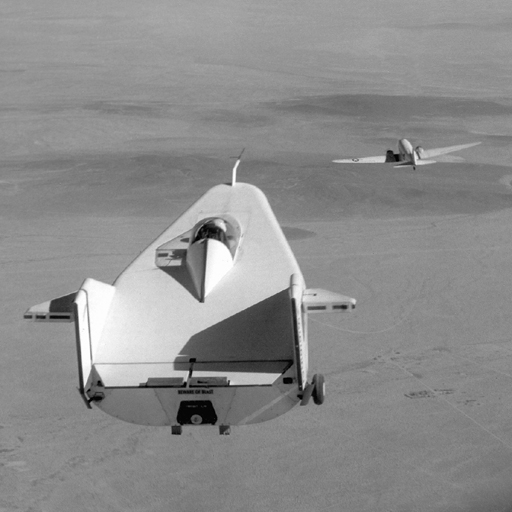
\includegraphics[width=\linewidth]{../liftingbody}
		\caption{Исходное изображение}
		\label{fig:liftingCurvedOriginal}
	\end{subfigure}
	\hfill
	\begin{subfigure}[t]{0.3\textwidth}
		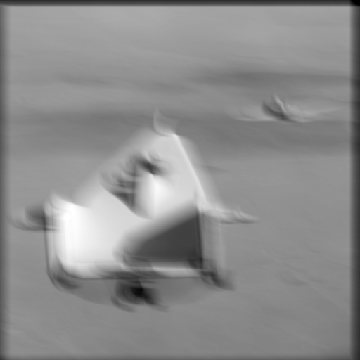
\includegraphics[width=\linewidth]{one-dim-iterated-blurred-data}
		\caption{смазанное изображение}
		\label{fig:liftingCurvedBlurred}
	\end{subfigure}
	\hfill
	\begin{subfigure}[t]{0.3\textwidth}
		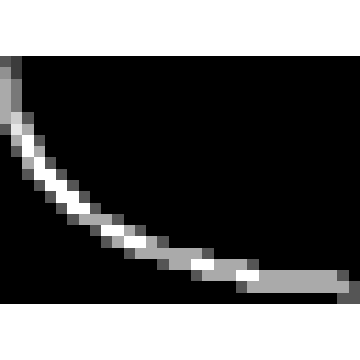
\includegraphics[width=\linewidth]{one-dim-iterated-curved-psf-real}
		\caption{кривая Безье второго порядка, построенной по точкам $B_0=(0; 0), B_1=(1; 18), B_2=(30; 20)$}
		\label{fig:curvedPsf}
	\end{subfigure}
	\caption{Смаз изображения криволинейным оператором}
\end{figure}

На рисунке~\ref{fig:curvedPsf} показана импульсная характеристика искажающего оператора представленная кривой Безье второго порядка, а на рисунке \ref{fig:liftingCurvedBlurred}~--- изображение смазанное, этим оператором.

\subsection{Первое приближение}
\begin{figure}[h!]
	\begin{subfigure}[t]{0.5\textwidth}
		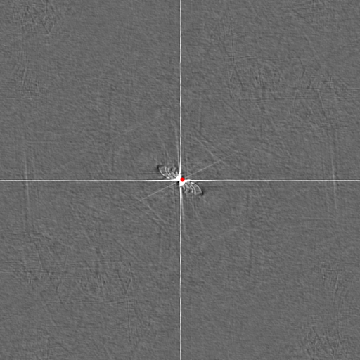
\includegraphics[width=\linewidth]{one-dim-iterated-kepstr}
		\caption{кепстр изображения \ref{fig:liftingCurvedBlurred}}
		\label{fig:curvedKepstrUnmodified}
	\end{subfigure}
	\begin{subfigure}[t]{0.5\textwidth}
		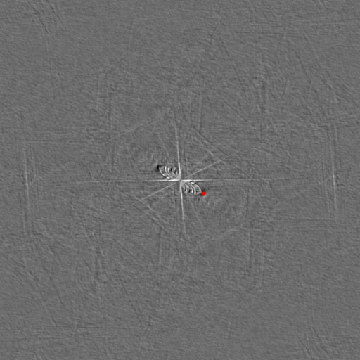
\includegraphics[width=\linewidth]{one-dim-iterated-kepstr-with-guass}
		\caption{сумма кепстра изображения \ref{fig:liftingCurvedBlurred} и гауссовой маски с $\sigma=3$}
		\label{fig:curvedKepstrWithGauss}
	\end{subfigure}
	\caption{Кепстр изображения с выделенным минимумом}
	\label{fig:}
\end{figure}

Итак, будем приближать искажающий оператор кривой Безье второго порядка. Следовательно, для полного задания оператора достаточно определить координаты трёх точек $B_0, B_1, B_2$ задающих кривую. Так как искажение инвариантно к смещению, то первую точку зафиксируем в нуле $B_0 = (0;0)$.

Точку $B_2$ попробуем приблизить применив метод из предыдущего раздела. На рисунке \ref{fig:curvedKepstrUnmodified} визуально определяются минимумы в тёмных точках вблизи нуля и на определённом расстоянии. Однако, абсолютный минимум(отмечен красной точкой) вблизи нуля не является искомой точкой. Для подавления некорректных минимумов применим высокочастотный фильтр Гаусса~(\ref{eq:gaussKernel})~\cite{basicsOfDigitalDIP200}.
\begin{equation}\label{eq:gaussKernel}
	W(x,y) = 1 - e^{-\frac{D^2(x,y)}{2D_0^2}},
\end{equation}
где $D_0$~--- масштабирующий параметр выбираемый эмпирически.

На модифицированном таким образом кепстре (рисунок~\ref{fig:curvedKepstrWithGauss}) корректно обнаруживается минимум, соответствующий кривой $B_2=(x_3,y_3)$. Первое приближение точки $B_1$ можно поместить посередине полученного отрезка.

\subsection{Второе приближение}
Для оценки $B_1$ построим целевую функцию $\psi(x,y)$ и будем её минимизировать. В качестве целевой функции возьмём:
\begin{equation}\label{eq:costFunction}
	\psi(x_2,y_2) = \left\|g - \phi(g, \hat{h}_{x_2,y_2}) \conv \hat{h}_{x_2,y_2}\right\|^2,
\end{equation}
где $h_{x_2,y_2}$~--- искажающий оператор представляющий собой кривую Безье построенную по точкам $b_0=(0;0), B_1=(x_2;y_2), B_2=(x_3;y_3)$. Здесь $x_3, y_3$~--- координаты третьей точки, полученные путём анализа кепстра(см. предыдущий подраздел). Минимизация данной функции означает, что будет выбран такой искажающий оператор, чтобы изображение восстановленное с его помощью и затем искажённое им же, было наиболее похожим на входное смазанное изображение.

Однако, данная целевая функция имеет множество локальных минимумов, что можно увидеть на рис.~\ref{fig:costFunctionGrid} (темнее~--- значение меньше), где изображена целевая функция для изображения смазанного по кривой Безье $B_0=(0;0), B_1=(15;4), B_2=(20, 20)$. Поэтому классические градиентные методы здесь плохо применимы.
\begin{figure}[h!]
	\centering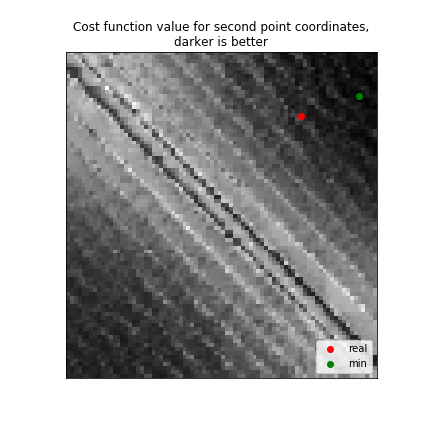
\includegraphics[width=0.5\linewidth]{cgrid-optimization_useless_x4}
	\caption{Значения целевой функции в зависимости от координат второй точки кривой}
	\label{fig:costFunctionGrid}
\end{figure}

Начальное приближение $B_1$ будем искать на серединном перпендикуляре между $B_0$ и $B_2$. Так как это задача одномерной минимизации, допустимо применение метода перебора по дискретной сетке с достаточно малым шагом $\alpha$ среди точек $B_1^i = \alpha i \vec{n}+\frac{B_0+B_2}{2}$, где $i = 0, \pm 1, \pm 2, \dots$; а $\vec{n}$~--- вектор нормали к прямой $B_0,B_2$.

\subsection{Уточнение параметров}
Для качественного восстановления изображения необходимо получить как можно более более точную оценку параметров искажения. Для чего применим метод наискорейшего спуска, начиная с полученных ранее оценок значений. Полученный таким образом минимум целевой функции может сойтись в глобальном минимуме. Как следствие получим качественно восстановленное изображение.

Метод наискорейшего спуска:
\begin{enumerate}
	\item Задать начальное приближение $X_0$
	\item Рассчитать $X_{j+1} = X_j - \lambda_j \nabla F(X_j)$, где $\lambda_j = \argmin_{\lambda} F(X_j - \lambda\nabla F(X_j))$
	\item Если $|X_{j+1}-X_j| > \varepsilon$, то $j = j+1$, иначе $X = X_j$ и останов.
\end{enumerate}

Так как целевая функция зашумлена, на втором шаге при вычислении градиента $\nabla F(x,y) = \left(\frac{\partial F(x,y)}{\partial x}, \frac{\partial F(x,y)}{\partial y}\right)$, вместо частных производных воспользуемся дискретным приближением~--- оператором Собел. Так его компонента по x:
\begin{equation*}
	\begin{aligned}
		G_x(x,y) = &-F(x-1, y-1) - 2F(x-1, y) - F(x-1, y+1) + \\
                   &+F(x+1, y-1) + 2F(x+1, y) + F(x+1, y+1)
	\end{aligned}
\end{equation*}
Таким образом можно получить достаточно точную оценку искажающего оператора, если он не является слишком сложной кривой.

Итоговый алгоритм оценки параметров искажения:
\begin{algorithm} Определение параметров криволинейного искажающего оператора
	
	\textbf{Входные данные:} искажённое изображение

	\textbf{Выходные данные:} оценка параметров искажающего оператора $h(x,y)$, а именно точки кривой Безье $B_0, B_1, B_2$.
	\begin{enumerate}
		\item Зафиксировать точку $B_0 = (0;0)$;
		\item Вычислить кепстр $\hat{g}(x,y)$ искажённого изображения;
		\item Произвести высокочастотную фильтрацию кепстра, фильтром Гаусса~(\ref{eq:gaussKernel});
		\item Начальное приближение точки $B_2^0 = \argmin_{b=(x,y)} \hat{g}(x,y)*\left(1 - e^{-\frac{D^2(x,y)}{2D_0^2}}\right)$;
		\item Начальное приближение точки $B_1$ выбирается перебором на серединном перпендикуляре между $B_0$ и $B_2$;
		\item Последовательное уточнение точек $B_1$ и $B_2$ методом наискорейшего спуска. 
	\end{enumerate}
	\label{algo:curve}
\end{algorithm}

\section{Выводы}
Были рассмотрены методы оценки параметров линейного и криволинейного искажающего оператора. Для каждого были сделаны выводы:
\begin{itemize}
	\item для деконволюции предлагается использовать модифицированный метод Люси-Ричардсона;
	\item кепстр позволяет достаточно точно определить параметры линейного искажающего оператора;
	\item по кепстру также можно сделать первое приближение третьей точки криволинейного искажающего оператора;
	\item составлен алгоритм оценки параметров криволинейного искажения.
\end{itemize}
\chapter{Результаты экспериментов}
\section{Оценка линейного искажающего оператора}
\section{Оценка криволинейного искажающего оператора}
\subsection{Искусственные искажения}
\subsection{Искажения <<от руки>>}
\section{Выводы}

\conclusion

Подводим заключение всей нашей эпопее по написанию ВКР.

Также в данном пункте можно вставить благодарности людям, помогавшим в написании работы: маме, дяде Феде с соседнего подъезда и коту.


%\bibliographystyle{ugost2008}
%\bibliography{biblio}
% Список литературы
\printbibliography[heading=bibintoc]

% Приложения
%\appendix
%\input{a}

\end{document}
